%% \begin{itemize}
%% \item We implemented the bi-LSTM transducer model using the \keras\ framework \cite{chollet2015} with a \tensorflow\ backend \cite{tensorflow2015-whitepaper}.
%%   We use 3 layers of stacked bi-LSTMs, where LSTM cell is composed of @ hidden units.
%%   for the LSTM we use

%%   \item Dimensions of layers
%%   \item activation functions
%%   \item Average perceptron part of speech tagging (as implemented in spaCy\footnote{\url{https://spacy.io}}
%%   \item Word embedding intialization using the pre-trained embeddings computed in
%%     \newcite{pennington2014glove}.
%% \end{itemize}

When evaluating Open IE it is desired to allow some room for flexibility when comparing against gold annotated extractions, for several reasons.
First, as we mentioned previously, current prominent Open IE systems were developed without a large reference
corpus. Following, this created some deviation in design and representation choices between the systems.
For example, ClausIE chooses to predict only binary extractions (versus n-ary extractions in the other systems), and PropS includes prepositions as part of the predicate while Open IE4 posits them in the respective
argument slot.

Second, like other tasks that require subtle semantic decisions, such as summarization or machine translation,
there are often several possible  extractions that might be regarded as correct, and we do not want to penalize systems for not
recovering the specific choice made in the gold corpus.
For example, for the sentence \sent{The sheriff standing against the wall spoke in a very soft voice} the two following
extractions can be considered acceptable: \extraction{The Sheriff}{spoke}{in a soft voice},
\extraction{The sheriff standing against the wall}{spoke}{in a very soft voice}

To account for  this variance in predictions, we follow \newcite{hequestion} and \newcite{Stanovsky2016EMNLP} which judge an argument as correct if and only if it includes the \emph{syntactic head} of the gold argument.%\footnote{We make use of the test suite published in \url{https://github.com/gabrielStanovsky/oie-benchmark}}
This would accept both variations of the previous example.
Note that this relaxed matching allows for fair comparison with rule-based systems which did not use a training
set to fit their prediction according to a strict matching function.

\subsection{Results}

%% \pgfplotsset{
	compat=1.5, 
	label style={font=\footnotesize},
	legend style={font=\footnotesize},
	every tick label/.append style={font=\tiny},
}



\begin{figure}  

\vspace{-2mm}
\centering

\begin{tikzpicture}
  \begin{axis}[
  ybar,
  bar width=2pt,
  xtick=data,% crucial line for the xticklabels directive
   xticklabels from table={../evaluations/figures/joint/predicate/auc.dat}{system}
  ]
        \addplot[red,mark size=0pt] table [x=auc] {../evaluations/figures/joint/predicate/auc.dat};
  \end{axis}
\end{tikzpicture}

\caption{AUC Predicate identification @}
\label{fig:rascal}



\end{figure}

%% %% https://tex.stackexchange.com/questions/21220/using-labels-from-a-file-in-pgfplot
%% https://tex.stackexchange.com/questions/103301/horizontal-bargraph-pgfplot

\pgfplotsset{
	compat=1.5,
	label style={font=\footnotesize},
	legend style={font=\footnotesize},
	every tick label/.append style={font=\tiny},
        every node near coord/.style={font=\tiny}
}



\begin{figure}  
\centering
\vspace{-2mm}
\centering

\begin{tikzpicture}
  \begin{axis}[
  width = 0.9\linewidth,
  height=3cm,
  xbar,
  xmax = 0.7,
  bar width=2pt,
  ytick=data,% crucial line for the xticklabels directive
   yticklabels from table={../evaluations/figures/joint/arguments/auc.dat}{system},
nodes near coords,
nodes near coords align={horizontal}
  ]
        \addplot[draw=blue,fill=blue!80!white,mark size=0pt] table [x=auc, y expr=\coordindex] {../evaluations/figures/joint/arguments/auc.dat};
  \end{axis}
\end{tikzpicture}

\caption{AUC Predicate identification @}
\label{fig:rascal}



 \end{figure}

%% \begin{tikzpicture}
%% \begin{axis}[
%% xbar, xmin=0,
%% xlabel={Percentage \%},
%% symbolic y coords={%
%%     {Bloodstream Infection (BSI)},
%%         {Surgical site infections (SSI)},
%%             {Ventilator-associated pneumonia (VAP)},
%%                 {Urinary tract infection (UTI)},
%%                     Others},
%%                     ytick=data,
%%                     nodes near coords,
%%                     nodes near coords align={horizontal},
%%                     ytick=data,
%%                     ]
%%                     \addplot coordinates {
%%                         (14,{Bloodstream Infection (BSI)})
%%                             (17,{Surgical site infections (SSI)})
%%                                 (14,{Ventilator-associated pneumonia (VAP)})
%%                                     (33,{Urinary tract infection (UTI)})
%%                                         (22,Others)};
%%                                         \end{axis}
%%                                         \end{tikzpicture} %width=6cm,height=7.59cm

%% %% https://tex.stackexchange.com/questions/21220/using-labels-from-a-file-in-pgfplot
%% https://tex.stackexchange.com/questions/103301/horizontal-bargraph-pgfplot

\pgfplotsset{
	compat=1.5,
	label style={font=\footnotesize},
	legend style={font=\footnotesize},
	every tick label/.append style={font=\tiny},
        every node near coord/.style={font=\tiny}
}



\begin{figure}  
\centering
\vspace{-2mm}
\centering

\begin{tikzpicture}
  \begin{axis}[
  width = 0.9\linewidth,
  height=3cm,
  xbar,
  xmax = 0.5,
  bar width=2pt,
  ytick=data,% crucial line for the xticklabels directive
   yticklabels from table={../evaluations/figures/joint/auc.dat}{system},
nodes near coords,
nodes near coords align={horizontal}
  ]
        \addplot[draw=blue,fill=blue!80!white,mark size=0pt] table [x=auc, y expr=\coordindex] {../evaluations/figures/joint/auc.dat};
  \end{axis}
\end{tikzpicture}

\caption{AUC Predicate identification @}
\label{fig:rascal}



 \end{figure}

%% \begin{tikzpicture}
%% \begin{axis}[
%% xbar, xmin=0,
%% xlabel={Percentage \%},
%% symbolic y coords={%
%%     {Bloodstream Infection (BSI)},
%%         {Surgical site infections (SSI)},
%%             {Ventilator-associated pneumonia (VAP)},
%%                 {Urinary tract infection (UTI)},
%%                     Others},
%%                     ytick=data,
%%                     nodes near coords,
%%                     nodes near coords align={horizontal},
%%                     ytick=data,
%%                     ]
%%                     \addplot coordinates {
%%                         (14,{Bloodstream Infection (BSI)})
%%                             (17,{Surgical site infections (SSI)})
%%                                 (14,{Ventilator-associated pneumonia (VAP)})
%%                                     (33,{Urinary tract infection (UTI)})
%%                                         (22,Others)};
%%                                         \end{axis}
%%                                         \end{tikzpicture} %width=6cm,height=7.59cm


\pgfplotsset{
	label style={font=\footnotesize},
	legend style={font=\footnotesize},
	every tick label/.append style={font=\tiny},
        every node near coord/.style={font=\tiny},
        every axis plot/.append style={line width = 0.6pt}
}



\begin{figure}[!ht]
    \centering
\begin{tikzpicture}
%%% ALL
\begin{axis}[
	xlabel=Recall,
        xticklabel pos=right,
	ylabel=Precision,
%	ymin=0,
	ymax=1,
        xmin=0,
        xmax=1,
	%ytick distance=.1,
%	height=0.25\textheight,
	width=0.33\textwidth,
	axis lines=left,
	%% legend entries={RnnOIE,OpenIE-4,PropS,ClausIE},
	%% legend style={draw=none,font=\tiny,at={(1,0.01)}, anchor=south east},
         /pgf/number format/.cd,
        1000 sep={}
]
\addplot[color1,mark size=0pt] table [x=Recall,y=Precision] {../../evaluations/figures/joint/RnnOIE.dat} node[right,pos=1] {\tiny RnnOIE};
\addplot[color2,mark size=0pt] table [x=Recall,y=Precision] {../../evaluations/figures/joint/OpenIE-4.dat} node[left,pos=1] {\tiny OpenIE-4};
\addplot[color3,mark size=0pt] table [x=Recall,y=Precision] {../../evaluations/figures/joint/PropS.dat} node[below,pos=0.7] {\tiny PropS};
\addplot[color4,mark size=0pt] table [x=Recall,y=Precision] {../../evaluations/figures/joint/ClausIE.dat} node[above,pos=1] {\tiny ClausIE};
\end{axis}
\end{tikzpicture}
%% \renewcommand{\thesubfigure}{a}
%% \subfloat[\small{Full Open-IE: PR and AUC.}]{
%% \label{fig:prop}
    \begin{tikzpicture}
  \begin{axis}[
  width = 0.4\textwidth,
  height=5cm,
  xbar,
  xmax = 0.49,
  bar width=2pt,
  xtick= \empty,
  ytick=data,% crucial line for the xticklabels directive
   yticklabels from table={../../evaluations/figures/joint/auc.dat}{system},
nodes near coords,
nodes near coords align={horizontal}
  ]
        \addplot[draw=blue,fill=blue!80!white,mark size=0pt] table [x=auc, y expr=\coordindex] {../../evaluations/figures/joint/auc.dat};
  \end{axis}
\end{tikzpicture}
%% $\;$
%% \renewcommand{\thesubfigure}{b}
%% \subfloat[\small{Predicate extraction: PR and AUC.}]{
%% \label{fig:pred}
%%     \begin{tikzpicture}
%%   \begin{axis}[
%%   width = 0.3\textwidth,
%%   height=3cm,
%%   xbar,
%%   xmax = 0.62,
%%   bar width=2pt,
%%   ytick=data,% crucial line for the xticklabels directive
%%    yticklabels from table={../evaluations/figures/joint/predicate/auc.dat}{system},
%% nodes near coords,
%% nodes near coords align={horizontal}
%%   ]
%%         \addplot[draw=blue,fill=blue!80!white,mark size=0pt] table [x=auc, y expr=\coordindex] {../evaluations/figures/joint/predicate/auc.dat};
%%   \end{axis}
%% \end{tikzpicture}

%%     }
%%     $\;$
%% \renewcommand{\thesubfigure}{c}
%% \subfloat[\small{Argument extraction: PR and AUC.}]{
%% \label{fig:arg}
%%     \begin{tikzpicture}
%%   \begin{axis}[
%%   width = 0.3\textwidth,
%%   height=3cm,
%%   xbar,
%%   xmax = 0.71,
%%   bar width=2pt,
%%   ytick=data,% crucial line for the xticklabels directive
%%    yticklabels from table={../evaluations/figures/joint/arguments/auc.dat}{system},
%% nodes near coords,
%% nodes near coords align={horizontal}
%%   ]
%%         \addplot[draw=blue,fill=blue!80!white,mark size=0pt] table [x=auc, y expr=\coordindex] {../evaluations/figures/joint/arguments/auc.dat};
%%   \end{axis}
%% \end{tikzpicture}
%% }
%%     %% \qquad
%%     %% \subfloat[Figura 3]{
%%     %%     
\includegraphics[width=0.4\columnwidth]{./figures/lorem-ipsum.jpg}
%%     %% }
%%     \caption{Precision-recall curves of the different systems on Open IE's subtasks (top),
%%     and corresponding areas under the curve (bottom)  -- complete Open IE (predicate-argument extraction) (\ref{fig:prop}),
%%     predicate extraction (\ref{fig:pred}), and argument extraction (\ref{fig:arg}).
%%     See details in Section \ref{sec:analysis}.
%%     }
%%     \label{fig:subfigname}
\end{figure}



%% \pgfplotsset{
	compat=1.5, 
	label style={font=\footnotesize},
	legend style={font=\footnotesize},
	every tick label/.append style={font=\tiny},
}



\begin{figure}  

\vspace{-2mm}
\centering
\begin{tikzpicture}
\begin{axis}[
	xlabel=Recall,
	ylabel=Precision,
	ymin=0,
	ymax=1,
        xmin=0,
        xmax=1,
	%ytick distance=.1,
	height=0.25\textheight,
%	width=\columnwidth,
	axis lines=left,
	legend entries={RnnOIE,OpenIE-4,PropS,ClausIE},
	legend style={draw=none,font=\tiny,at={(1,0.01)}, anchor=south east},
         /pgf/number format/.cd,
        1000 sep={}
]

\addplot[red,mark size=0pt] table [x=Recall,y=Precision] {../evaluations/figures/joint/predicate/RnnOIE.dat};
\addplot[brown,mark size=0pt] table [x=Recall,y=Precision] {../evaluations/figures/joint/predicate/OpenIE-4.dat};
\addplot[orange,mark size=0pt] table [x=Recall,y=Precision] {../evaluations/figures/joint/predicate/PropS.dat};
\addplot[blue,mark size=0pt] table [x=Recall,y=Precision] {../evaluations/figures/joint/predicate/ClausIE.dat};

\end{axis}
\end{tikzpicture}
\caption{Predicate identification @}
\label{fig:rascal}



\end{figure}

%% \pgfplotsset{
	compat=1.5, 
	label style={font=\footnotesize},
	legend style={font=\footnotesize},
	every tick label/.append style={font=\tiny},
}



\begin{figure}  

\vspace{-2mm}
\centering
\begin{tikzpicture}
\begin{axis}[
	xlabel=Recall,
	ylabel=Precision,
	ymin=0,
	ymax=1,
        xmin=0,
        xmax=1,
	%ytick distance=.1,
	height=0.25\textheight,
%	width=\columnwidth,
	axis lines=left,
	legend entries={RnnOIE,OpenIE-4,PropS,ClausIE},
	legend style={draw=none,font=\tiny,at={(1,0.01)}, anchor=south east},
         /pgf/number format/.cd,
        1000 sep={}
]

\addplot[red,mark size=0pt] table [x=Recall,y=Precision] {../evaluations/figures/joint/arguments/RnnOIE.dat};
\addplot[brown,mark size=0pt] table [x=Recall,y=Precision] {../evaluations/figures/joint/arguments/OpenIE-4.dat};
\addplot[orange,mark size=0pt] table [x=Recall,y=Precision] {../evaluations/figures/joint/arguments/PropS.dat};
\addplot[blue,mark size=0pt] table [x=Recall,y=Precision] {../evaluations/figures/joint/arguments/ClausIE.dat};

\end{axis}
\end{tikzpicture}
\caption{Arguments @}
\label{fig:rascal}



\end{figure}

 \pgfplotsset{
	compat=1.5, 
	label style={font=\footnotesize},
	legend style={font=\footnotesize},
	every tick label/.append style={font=\tiny},
}



\begin{figure}  

\vspace{-2mm}
\centering
\begin{tikzpicture}
\begin{axis}[
	xlabel=Recall,
	ylabel=Precision,
	ymin=0,
	ymax=1,
        xmin=0,
        xmax=1,
	%ytick distance=.1,
	height=0.25\textheight,
%	width=\columnwidth,
	axis lines=left,
	legend entries={Seen in train,Unseen in train},
	legend style={draw=none,font=\tiny,at={(1,0.01)}, anchor=south east},
         /pgf/number format/.cd,
        1000 sep={}
]

\addplot[cyan, mark size=0pt] table [x=Recall,y=Precision] {../evaluations/only_in_test/seen.dat};
\addplot[purple,mark size=0pt] table [x=Recall,y=Precision] {../evaluations/only_in_test/unseen.dat};

\end{axis}
\end{tikzpicture}
\caption{Seen vs. Unseen @}
\label{fig:rascal}



\end{figure}



%% accuracy and attention comparison figures

\begin{figure*}[t!]

  \centering
  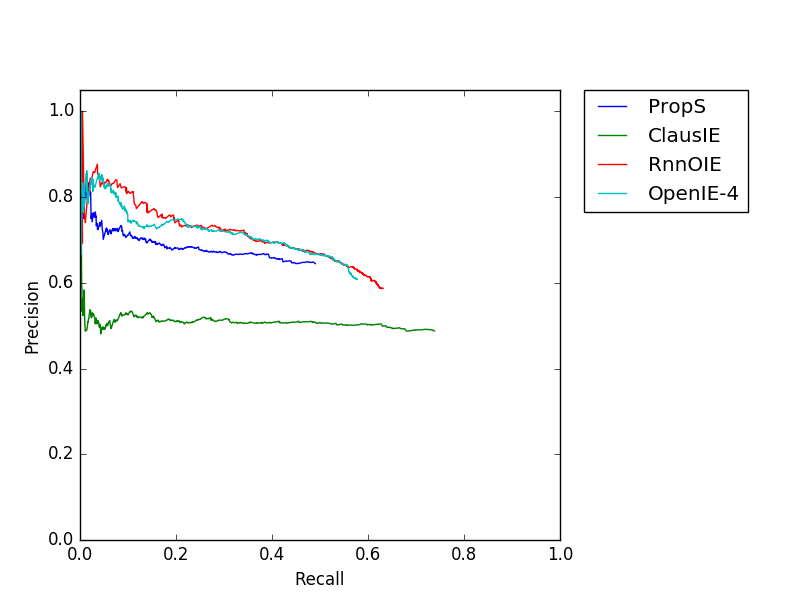
\includegraphics[width=.5\textwidth]{figures/joint/pr}\hfill
  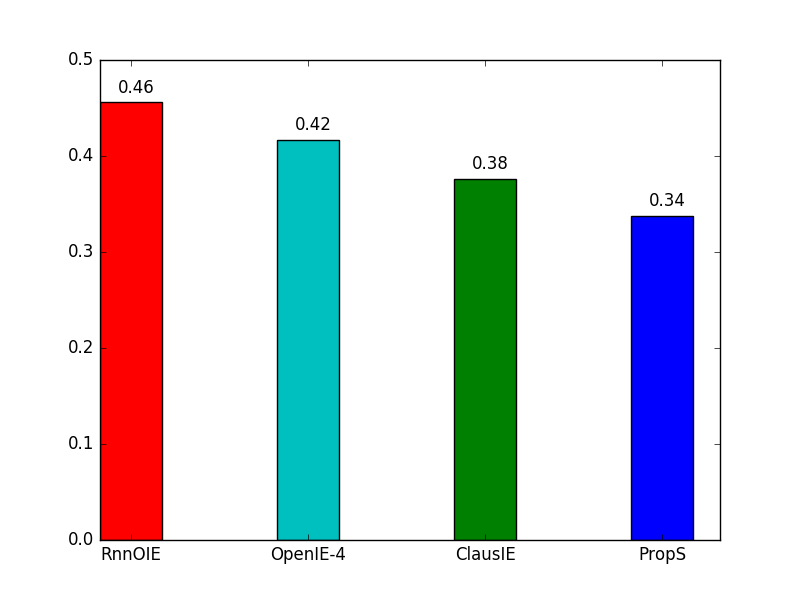
\includegraphics[width=.5\textwidth]{figures/joint/auc}

  \caption{Precision-Recall curve (left) and respective area under the curve (right) for the different systems.}
  \label{fig:evaluation}

\end{figure*}


%% \begin{figure*}[t!]

%%   \centering
%%   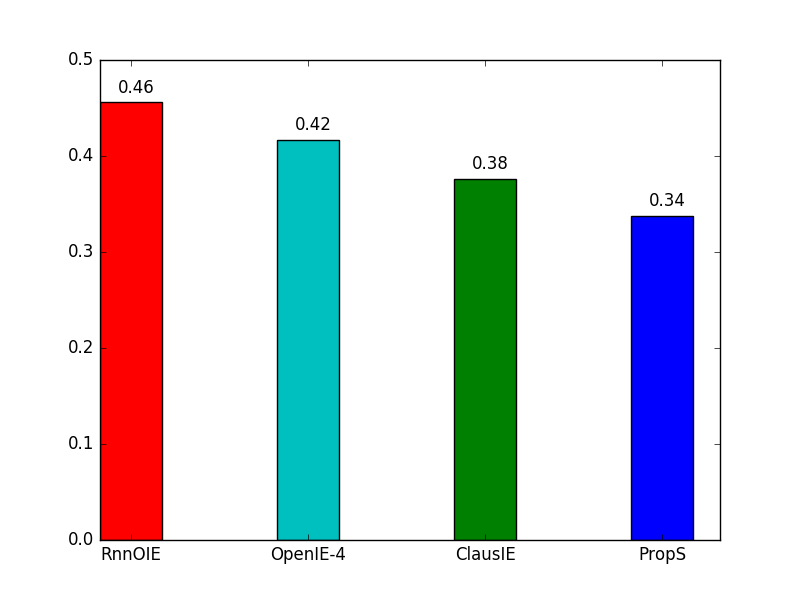
\includegraphics[width=.3\textwidth]{figures/joint/auc}\hfill
%%   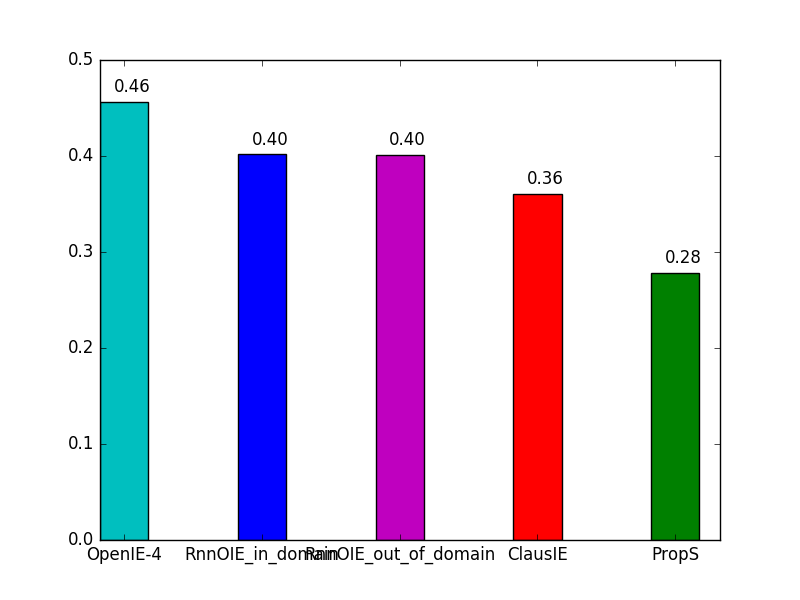
\includegraphics[width=.3\textwidth]{figures/newswire/auc}\hfill
%%     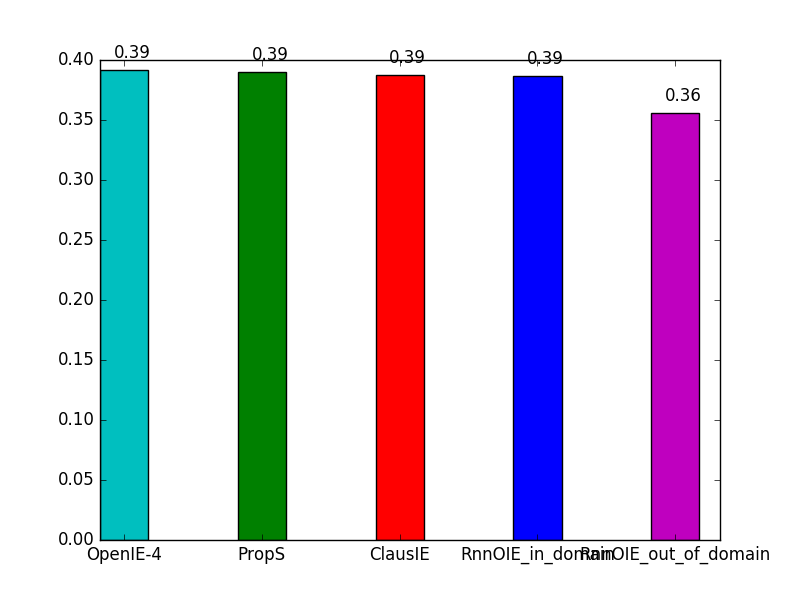
\includegraphics[width=.3\textwidth]{figures/wiki/auc}

%%   \caption{Area under the PR - curves for the entire test corpus (left), Newswire (middle), and Wikipedia (right).}
%%   \label{fig:figure3}

%% \end{figure*}



%% \begin{figure*}[!hb]

%%   \centering

%%   \begin{minipage}[b]{.12\textwidth}
%%     \begin{center}
%%       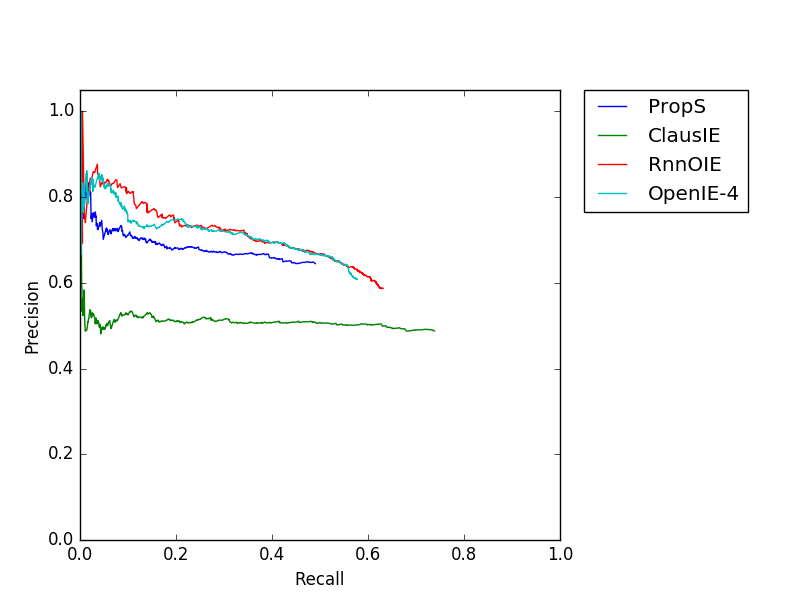
\includegraphics[width=\textwidth]{figures/joint/pr}
%%       \caption {Precision-recall curve on the full test partition}
%%       \label{fig:alignments}
%%     \end{center}
%%   \end{minipage}

%%   \begin{minipage}[b]{0.12\textwidth}
%%     \begin{center}
%%       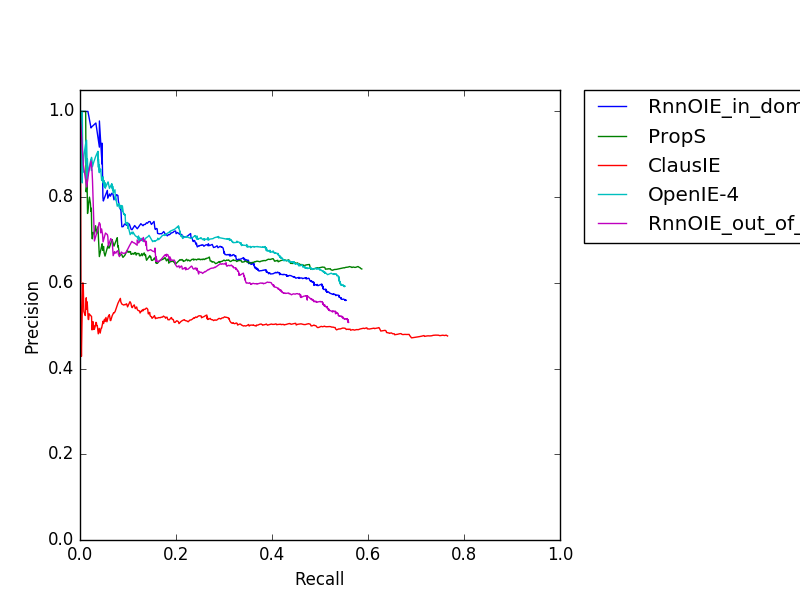
\includegraphics[width=\textwidth]{figures/wiki/pr}
%%       \caption {Precision-recall curve on the Wikipedia test partition}
%%       \label{fig:alignments}
%%     \end{center}
%%   \end{minipage}

%%   \begin{minipage}[b]{0.12\textwidth}
%%     \begin{center}
%%       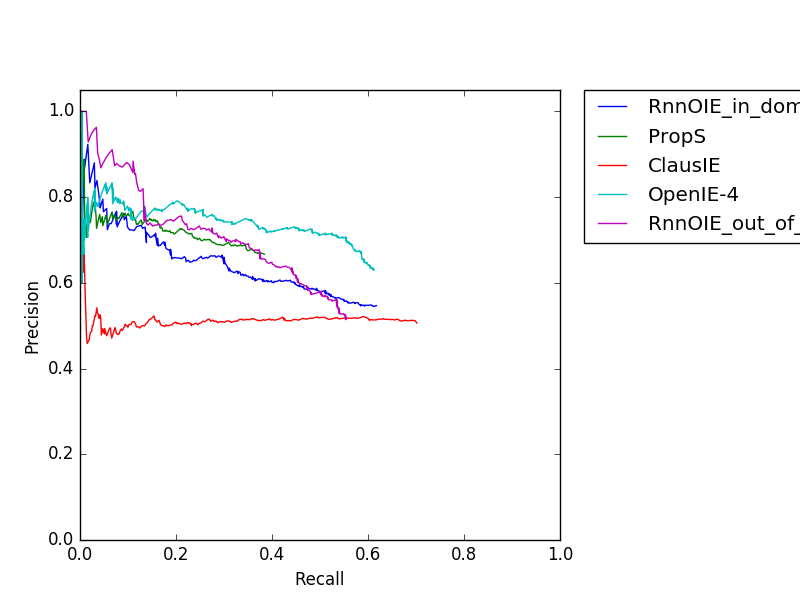
\includegraphics[width=\textwidth]{figures/newswire/pr}
%%       \caption {Precision-recall curve on the newswire test partition}
%%       \label{fig:alignments}
%%     \end{center}
%%   \end{minipage}


%% \end{figure*}


The Precision-Recall (PR) curve of our model (marked RnnOIE) is shown in Figure \ref{fig:prop},
using the soft matching function discussed above.
For comparison, we plot the performance of the top performing systems evaluated in \cite{Stanovsky2016EMNLP} on the same corpus. We note that these are very strong baseline systems, which are the result of over a decade of research.

RnnOIE outperforms the other systems in terms of precision on most of the recall range, and comes in second after (the much less precise) ClausIE in terms of maximum obtained recall (.63 versus .74).
Superior precision performance is especially attractive for
applications that employ Open IE over large amounts of data, in which a high degree of data redundancy is expected, such as in different news reports of the same event.

Following, the Area Under the PR-Curve (AUC), depicted below the PR curve, shows that overall our system
produces the best combination of aggregated precision and recall with a statistically significant margin over
the other systems. Furthermore, in scalar terms of the AUC, our improvement over state-of-the-art is similar in magnitude to previous
advancements in the field (roughly 4 points).


%\todo{it's worth mentioning the statistical test used}

%% \begin{itemize}
%% \item Figures:
%%   \begin{itemize}
%%   \item Optimizing precision vs. recall.
%%   \item In \& Out of domain?
%%   \item Number of extractions per system
%%   \item Check whether its common to report ``intrinsic'' numbers
%%   \end{itemize}
%% \end{itemize}

\subsection{Analysis}
\label{sec:analysis}
We describe several observations about the performance of the evaluated systems.

\paragraph{RnnOIE outperforms the baselines at both predicate and argument extraction.}
We analyze the systems' performance on two complementing subtasks of Open IE:
(1) \emph{Predicate extraction} (Figure \ref{fig:pred}), which evaluates the systems' ability to correctly recover the predicate slot, and
(2) \emph{Argument extraction} (Figure \ref{fig:arg}), which evaluates their recovery of the argument slots.

This analysis shows that RnnOIE performs best (in terms of AUC) on both subtasks.
Particularly, it most significantly outperforms the other systems on the task of predicate extraction.
We hypothesize that this is since predicates are allotted a different label, and that
the predicate label is the only one which must inherently appear in every training sample.


\paragraph{RnnOIE is able to generalize to unseen predicates.}
We analyze the extent to which our model overfits for the predicates seen during training, that is, whether it achieves good performance by memorizing specific patterns for these predicates.
To that end we have split the propositions in the gold and predicted test set into two corresponding partitions, namely ``seen'' and ``unseen'',
based on whether the predicate lemma appears in the training set or not.
The ``unseen'' part of the test set contains 145 unique predicate lemmas, constituting
24\% out of a total of 590 unique predicate lemmas in the entire test set.
Furthermore, it is composed of a total of 148 propositions (7\% out of 1993 in the entire test).
%% \todo{the above sentence isn't so clear, not sure what you meant to say. Do you refer to the fact that in 148 unseen propositions there were 145 different predicates? This isn't that surprising - events not seen in training are rare and are likely to be singletons in test. If that's the case maybe you can drop this sentence on the variability, not sure if it contributes to the main point here on unseen}

Following, we tested each of the predicted test partitions against its corresponding gold
counterpart.
The resulting PR curves (Figure \ref{fig:unseen}) depict overall good performance on the ``unseen'' partition,
We note, however, that the ``seen'' part is much larger, constituting roughly 93\% of the test data.
Overall, this indicates that the model indeed generalizes beyond the memorization of specific predicate templates, as
it managed to predict extractions for unseen predicates with good accuracy.


\begin{table}[tb!]
  \centering
  \resizebox{1\columnwidth}{!}{
    \begin{tabular}{@{}lrrr@{}}
      \toprule
      \multirow{2}{*}{\textbf{System}} & \multicolumn{1}{l}{\multirow{2}{*}{\textbf{\# Extractions}}} & \multicolumn{1}{l}{\multirow{2}{*}{\textbf{Arg. per Prop.}}} & \multicolumn{1}{l}{\multirow{2}{*}{\textbf{Words per Arg}}} \\
      & \multicolumn{1}{l}{} & \multicolumn{1}{l}{} & \multicolumn{1}{l}{} \\ \midrule
      Gold & 1730 & 2.45 & 26.91 \\ \midrule
      ClausIE & 2768 & 2.00 & 28.89 \\
      Open IE4 & 1793 & 3.07 & 22.75 \\
      PropS & 1551 & 2.68 & 29.00 \\
      RnnOIE & 1993 & 3.19 & 23.40 \\ \bottomrule
      \end{tabular}
  }
  \caption{Output statistics of the different systems.}
  \label{tab:output_stats}
  \end{table}


\paragraph{RnnOIE and Open IE4 produce shorter arguments.}
In Table \ref{tab:output_stats} we examine some properties of the output of the systems compared to the corresponding characteristics of the gold data.
This allows us to gain some insight into the performance of the systems.
For example, we can see that the best performing systems (RnnOIE and OpenIE4), tend to produce
more arguments, each of which tending to be shorter in terms of word count.
This observation fits the \emph{minimality} principle of Open IE, discussed in Section \ref{sec:background}.
Comparing to the same properties in the gold data set (first row), we can see that both systems
tend to overproduce and over-shorten their arguments.
% Compared to 2.45 arguments of 26.91 word length in average for the gold data set,
% RnnOIE and Open IE4 produce 3.07 and 3.19 arguments of word length 23.4 and 22.75 in average, respectively.


%% \begin{figure}[tb!]

%%   \centering
%%     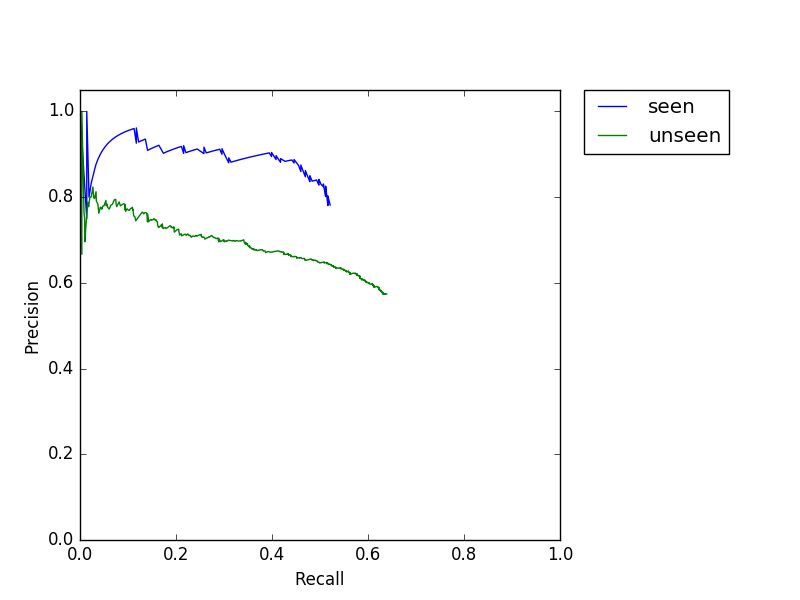
\includegraphics[width=1\columnwidth]{figures/uniq_test_pr}

%%   \caption{Performance of our model on seen versus unseen test predicates.}
%%   \label{fig:unseen}

%% \end{figure}


%% \begin{itemize}
%% \item Performace on ``core'' arguments vs. ``adjuncts''
%% \item Standard error analysis: Sample 50 FN and 50 FP
%% \item Check what number of predicates are unseen in the test in each of these and do they affect performance
%% \end{itemize}
